\chapter{Discussion}

\section{Why Exposure Differs Across Profiles}

The results of this project suggest that dark pattern exposure in mobile applications is shaped by the interaction trajectory through which an interface is reached. A dark pattern may exist somewhere inside an application, but it becomes measurable exposure only when a profile enters the relevant interface state and receives a positive DPS label. This distinction matters because the controlled profiles in this project differ in both interest distributions and behavior distributions. They therefore generate different action sequences, and those action sequences lead to different estimates of \(E(D \mid A)\).

The high-payment shopping profile is more likely to enter decision-sensitive contexts. Its behavior distribution makes product search, product-detail inspection, cart entry, membership evaluation, and checkout-related actions more probable. These states are close to monetization and conversion, so they are also the states where Interface Interference, Pressure, Sneaking, Friction, and Forced Action may become visible. A checkout-adjacent screen may emphasize a purchase button, preselect an add-on, display a limited-time offer, or make refusal less salient. When such screens appear repeatedly in the trajectory, they raise the relevant components of \(E(D \mid A)\) and produce positive components in \(\Delta(A_i,A_j)\) against a lower-intent profile.

The bargain-hunter profile reaches a different but similarly sensitive set of contexts. Searches for coupons, group buying, discounts, limited offers, and promotional rewards move the trajectory toward interfaces where scarcity and urgency may be part of the service logic. In DPS terms, these contexts can activate Pressure and Interface Interference labels through countdowns, inventory warnings, visually dominant promotional buttons, reward thresholds, or messages that frame delay as loss. The observed results, however, show that Pressure is category-dependent rather than uniformly strongest for the bargain-hunter profile. The profile does not need to be treated as a demographic group for this mechanism to matter. It is enough that its keyword and action distributions increase the probability of entering promotion-heavy interface states.

By contrast, the low-payment browsing profile more often remains in feed, search, and general browsing states. These states can still contain dark patterns, especially Forced Action, Nagging, notification prompts, or login gates. However, they are less consistently tied to purchase conversion, coupon redemption, or payment decisions. The difference is therefore not a simple high-risk versus no-risk contrast. It is a difference in the distribution of observed DPS vectors across trajectory states.

This interpretation keeps the causal claim narrow. The audit observes profile-conditioned exposure, not the internal policy that produced each screen. Higher Interface Interference for a profile, or category-specific differences in Pressure, can arise from profile-driven navigation, content-conditioned recommendation, platform personalization, or their interaction. The empirical contribution is to show that the resulting exposure distributions differ in measurable ways, using \(E(D \mid A)\), \(\Delta(A_i,A_j)\), running mean stabilization, and permutation-based validation as evidence.

\section{Dark Pattern Exposure as a Distributional Problem}

A central implication of this project is that dark pattern exposure should be studied as a distributional problem rather than a static presence problem. Much existing work asks whether an application or website contains dark patterns, how those patterns can be categorized, and how frequently they appear in collected interface samples \cite{gray2018darkpatterns,mathur2019darkpatterns,mathur2021whatmakesdark}. That work is necessary for defining the phenomenon. However, the presence of a manipulative interface element somewhere in an application does not determine which users encounter it, how often they encounter it, or at what decision point it appears.

The DPS framework makes this distinction operational. Each screenshot is one observed interface state, represented as \(D_t=[I_t,F_t,P_t,C_t,S_t,N_t,FA_t]\). A profile-level estimate \(E(D \mid A)\) is not a claim that the app has a fixed amount of manipulation; it is the empirical mean of DPS observations produced by a profile-conditioned trajectory. Depending on the analysis, \(D_t\) can be the raw numeric score vector or the binarized occurrence vector \(1[D_t>0]\). The running mean curves further show why a single screenshot is not enough. Early observations can be dominated by onboarding, a login wall, or one promotional popup, while later estimates become more stable as the trajectory accumulates additional interface states.

This framing changes the research question. Instead of asking only whether a dark pattern exists, the audit asks how DPS labels are distributed across profiles, apps, categories, and steps. A forced login screen may appear only after a coupon action. A countdown may appear only in a discount-search path. A preselected membership benefit may appear only near checkout. A cancellation obstacle may appear only after a subscription path has already been entered. These are exposure conditions, not merely interface inventory items.

The distributional view also explains why \(\Delta(A_i,A_j)\), \(L_1\) distance, and permutation tests are useful. Pairwise differences identify which DPS dimensions separate two profiles. The \(L_1\) distance summarizes the magnitude of the vector-level gap. Permutation tests ask whether the observed gap is larger than would be expected after random profile-label reassignment. Together, these measures shift dark pattern auditing from static detection toward profile-conditioned exposure analysis, while still keeping the evidence tied to observable interface states.

\begin{figure}[htbp]
    \centering
    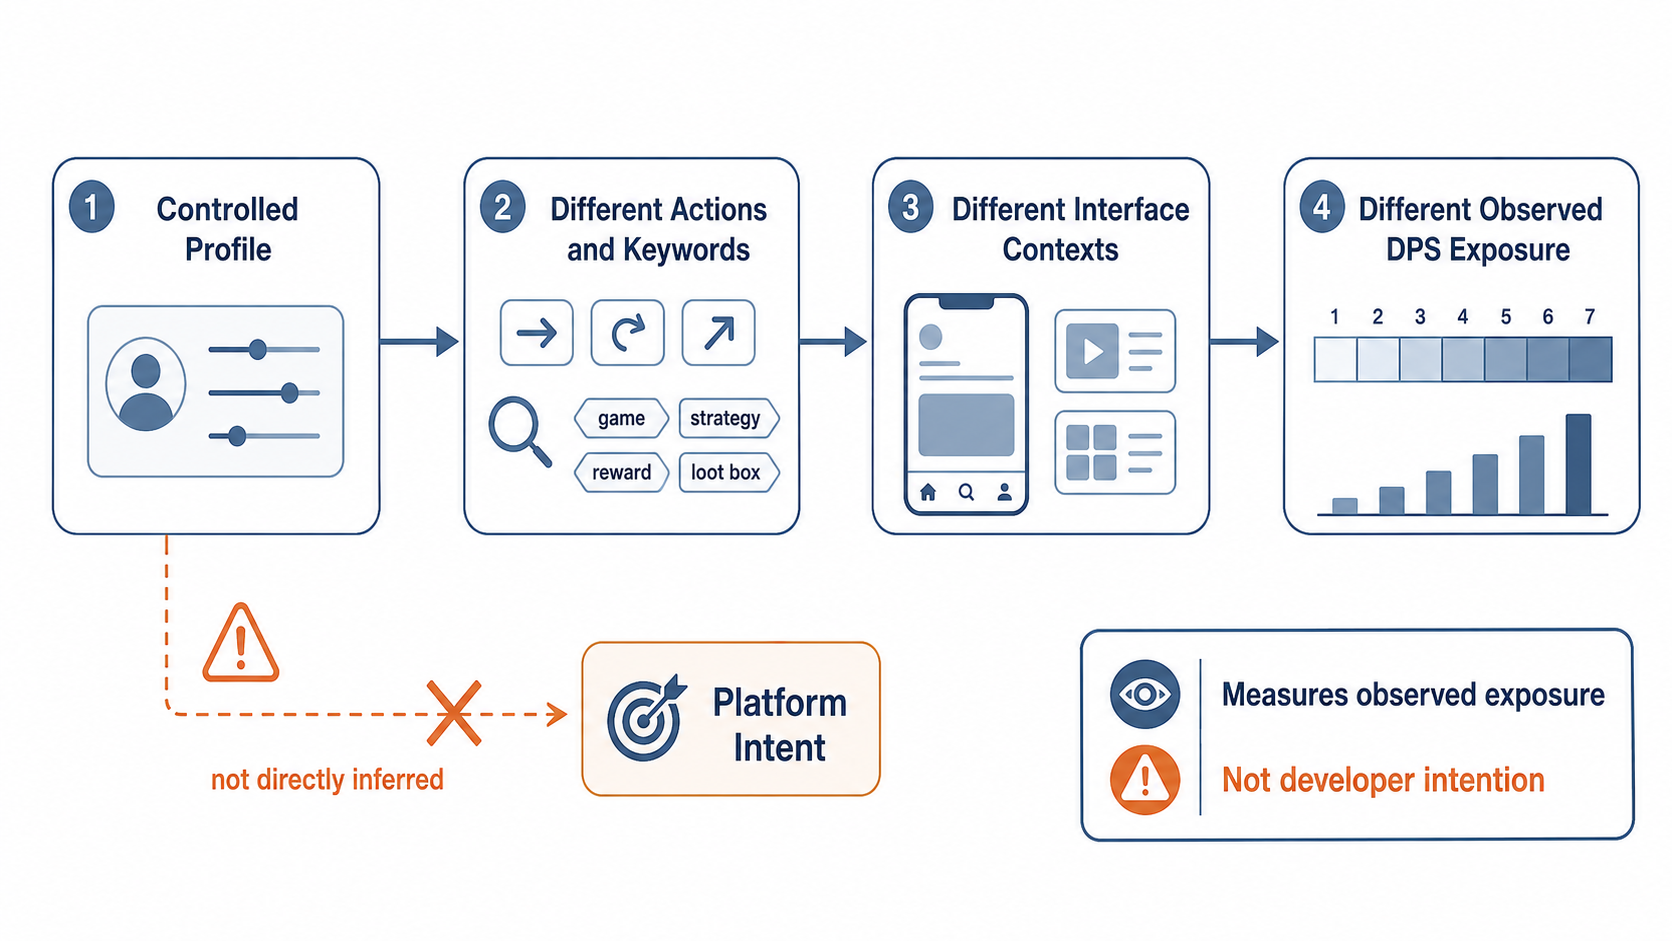
\includegraphics[width=0.95\linewidth]{figures/pictures/why_exposure_differs_across_profiles.png}
    \caption{Why Exposure Differs Across Profiles}
    \label{fig:why_exposure_differs_across_profiles}
\end{figure}

\section{Implications for Platform Accountability}

The distributional nature of dark pattern exposure has implications for platform accountability, but the implication is primarily methodological. Platforms should be evaluated not only by whether a dark pattern can be found, but by how DPS exposure is distributed across profile-conditioned trajectories. The relevant audit object is the exposure distribution \(E(D \mid A)\), together with profile gaps such as \(\Delta(A_i,A_j)\), rather than a single screenshot or a single default journey.

This framing avoids treating every profile difference as a moral accusation. Some differences are functionally expected. A profile that enters checkout more often will see more payment, membership, and delivery-choice interfaces. A profile that searches for coupons will see more promotion modules. The accountability question is whether these decision-sensitive contexts concentrate DPS mechanisms such as Pressure, Interface Interference, Sneaking, Friction, or Forced Action in ways that can be observed, measured, and compared across profiles.

A practical platform audit could therefore report profile-conditioned exposure distributions. Auditors could run the same application under high-payment, low-payment, bargain-seeking, and other controlled behavioral profiles; compute \(E(D \mid A, app)\) and \(E(D \mid A, category)\); compare profiles through \(\Delta(A_i,A_j)\) and \(L_1\) distance; and validate prominent gaps with permutation tests and corrected \(q\)-values. Such reporting would make clear whether a platform's pressure or interference exposure is broadly distributed, concentrated in purchase paths, concentrated in discount paths, or tied to access-control moments such as login and permissions.

The same logic can inform compliance and review processes. Sensitive flows such as subscription, payment, cancellation, coupon redemption, notification permission, and location permission should be audited as trajectories, not only as isolated screens. A platform-facing dashboard could track the running mean of each DPS dimension for major profile classes and flag cases where exposure remains elevated after repeated interaction steps. The goal of such tools is not to infer hidden intent from outside the system. It is to make profile-conditioned exposure measurable enough for review, comparison, and redesign.

\section{Implications for Users}

From the user perspective, the findings suggest that personal experience with an application may be an incomplete view of the platform's interface environment. A user sees the screens generated by their own trajectory, not the full distribution of screens that other profiles may encounter. If one user rarely enters checkout, they may underestimate payment-stage Pressure or Sneaking. If another user frequently searches for coupons, they may overestimate how central countdowns and scarcity messages are to the application as a whole.

High-payment users may face stronger commercial interface exposure because their behavior brings them closer to decision points. They may encounter membership prompts, limited-time offers, add-on recommendations, or interface designs that make payment-related actions visually salient while making refusal less convenient. In DPS terms, the relevant risk is not a single promotional screen, but repeated positive observations in dimensions such as Interface Interference, Pressure, Sneaking, or Friction across the trajectory.

Bargain hunters may face a different but related exposure pattern. Searches for discounts, coupons, flash sales, and promotional opportunities can increase contact with scarcity cues, countdown timers, social proof, and reward thresholds. These mechanisms can frame delay as loss or make benefits appear conditional on immediate participation. Because bargain-seeking behavior is often motivated by cost sensitivity, the category-specific distribution of pressure-heavy screens along this path deserves attention even when the same app also contains ordinary browsing interfaces.

Low-payment browsing users should not be treated as unaffected. They may avoid many checkout-specific screens, but still encounter Forced Action, repeated notification prompts, login gates, nagging pop-ups, permission requests, or friction when dismissing recommendations. Their \(E(D \mid A)\) may therefore be lower in some commercial dimensions while remaining meaningful in access-control or engagement-retention dimensions.

The broader lesson is that individual reports about an application's interface can be biased by trajectory. A user can accurately describe what they saw and still miss exposure patterns concentrated in other profile-conditioned paths. For this reason, user protection should not rely only on individual awareness or anecdotal comparison. It requires audits that sample multiple trajectories and estimate how DPS exposure is distributed across them.

\section{Implications for Researchers}

For researchers, this project suggests a bridge between dark pattern taxonomy and algorithm auditing. Dark pattern research provides the DPS vocabulary for identifying manipulative interface mechanisms, while audit methodology provides controlled procedures for comparing black-box outputs across profiles. The unit of analysis is therefore not only the screenshot, but the trajectory log that explains how the screenshot was reached.

Future work should strengthen three parts of this design. First, trajectory logging should record not only screenshots and DPS labels, but also actions, keywords, app states, timestamps, pop-up recurrence, dismissal attempts, and transitions into payment, subscription, coupon, permission, or cancellation flows. This would make it easier to distinguish decision-sensitive contexts from general browsing contexts and to interpret changes in the running mean over time.

Second, multi-profile auditing should be expanded beyond the three profiles used here while preserving experimental control. Additional profiles could vary purchase intent, coupon sensitivity, subscription history, permission refusal behavior, account age, or task goal. The purpose would not be to map demographic identity directly onto exposure, but to test how behaviorally defined profiles change \(E(D \mid A)\), \(E(D \mid A, app)\), and \(E(D \mid A, category)\).

Third, statistical validation should remain central. Pairwise differences \(\Delta(A_i,A_j)\) identify which DPS dimensions differ, but those differences should be evaluated with running mean stabilization, permutation tests, corrected \(q\)-values, \(L_1\) distance, and association measures such as Cramér's \(V\). This combination helps separate stable profile-conditioned patterns from isolated interface events or small-sample fluctuation.

More broadly, the project indicates that personalization and path dependence should become central concerns in dark pattern research. Static inspection can show that a manipulative design exists, but it cannot show how exposure is allocated across users and situations. By treating dark pattern exposure as profile-conditioned, measurable, and statistically testable, future research can study deceptive interfaces as dynamic components of personalized digital environments while keeping claims tied to observable evidence.
